\documentclass[10pt]{article}  

%%%%%%%% PREÁMBULO %%%%%%%%%%%%
\title{Plantilla para prácticas de UPIITA}
\usepackage[spanish]{babel} %Indica que escribiermos en español
\usepackage[utf8]{inputenc} %Indica qué codificación se está usando ISO-8859-1(latin1)  o utf8  
\usepackage{amsmath} % Comandos extras para matemáticas (cajas para ecuaciones,
% etc)
\usepackage{amssymb} % Simbolos matematicos (por lo tanto)
\usepackage{graphicx} % Incluir imágenes en LaTeX
\usepackage{color} % Para colorear texto
\usepackage{subfigure} % subfiguras
\usepackage{float} %Podemos usar el especificador [H] en las figuras para que se
% queden donde queramos
\usepackage{capt-of} % Permite usar etiquetas fuera de elementos flotantes
% (etiquetas de figuras)
\usepackage{sidecap} % Para poner el texto de las imágenes al lado
	\sidecaptionvpos{figure}{c} % Para que el texto se alinie al centro vertical
\usepackage{caption} % Para poder quitar numeracion de figuras
\usepackage{commath} % funcionalidades extras para diferenciales, integrales,
% etc (\od, \dif, etc)
\usepackage{cancel} % para cancelar expresiones (\cancelto{0}{x})
 
\usepackage{anysize} 					% Para personalizar el ancho de  los márgenes
\marginsize{2cm}{2cm}{2cm}{2cm} % Izquierda, derecha, arriba, abajo

\usepackage{appendix}
\renewcommand{\appendixname}{Apéndices}
\renewcommand{\appendixtocname}{Apéndices}
\renewcommand{\appendixpagename}{Apéndices} 

% Para que las referencias sean hipervínculos a las figuras o ecuaciones y
% aparezcan en color
\usepackage[colorlinks=true,plainpages=true,citecolor=blue,linkcolor=blue]{hyperref}
%\usepackage{hyperref} 
% Para agregar encabezado y pie de página
\usepackage{fancyhdr} 
\pagestyle{fancy}
\fancyhf{}
\fancyhead[L]{\footnotesize UGR} %encabezado izquierda
\fancyhead[R]{\footnotesize EV}   % dereecha
\fancyfoot[R]{\footnotesize Práctica IV}  % Pie derecha
\fancyfoot[C]{\thepage}  % centro
\fancyfoot[L]{\footnotesize Master en Ingeniería Informática}  %izquierda
\renewcommand{\footrulewidth}{0.4pt}

% Directorio para las imágenes
\graphicspath{{/Users/jesusgarciamanday/Desktop/Master/EV/Practicas/Practica4/p4/Imagenes/}}


\usepackage{listings} % Para usar código fuente
\definecolor{dkgreen}{rgb}{0,0.6,0} % Definimos colores para usar en el código
\definecolor{gray}{rgb}{0.5,0.5,0.5} 
% configuración para el lenguaje que queramos utilizar
\lstset{language=Matlab,
   keywords={break,case,catch,continue,else,elseif,end,for,function,
      global,if,otherwise,persistent,return,switch,try,while},
   basicstyle=\ttfamily,
   keywordstyle=\color{blue},
   commentstyle=\color{red},
   stringstyle=\color{dkgreen},
   numbers=left,
   numberstyle=\tiny\color{gray},
   stepnumber=1,
   numbersep=10pt,
   backgroundcolor=\color{white},
   tabsize=4,
   showspaces=false,
   showstringspaces=false}

\newcommand{\sen}{\operatorname{\sen}}	% Definimos el comando \sen para el seno
%en español

%%%%%%%% TERMINA PREÁMBULO %%%%%%%%%%%%

\begin{document}

%%%%%%%%%%%%%%%%%%%%%%%%%%%%%%%%%% PORTADA %%%%%%%%%%%%%%%%%%%%%%%%%%%%%%%%%%%%%%%%%%%%
																					%%%
\begin{center}																		%%%
\newcommand{\HRule}{\rule{\linewidth}{0.5mm}}									%%%\left
 																					%%%
\begin{minipage}{0.48\textwidth} \begin{flushleft}
%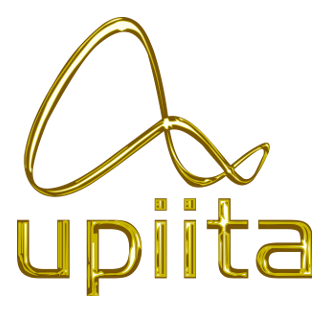
\includegraphics[scale = 0.63]{Imagenes/logo_upiita}
\end{flushleft}\end{minipage}
\begin{minipage}{0.48\textwidth} \begin{flushright}
%
\includegraphics[scale = 0.35]{Imagenes/IPN}
\end{flushright}\end{minipage}

													 								%%%
\vspace*{0.25cm}								%%%
																					%%%	
\textsc{\huge Universidad de Granada}\\[1.5cm]	

\textsc{\LARGE Master en Ingeniería Informática}\\[1.5cm]													%%%

\textsc{\LARGE Entornos Virtuales}\\[1.5cm]													%%%

\begin{minipage}{0.9\textwidth} 
\begin{center}																					%%%
\textsc{\LARGE Practica IV}
\end{center}
\end{minipage}\\[0.5cm]
%%%
    																				%%%
 			\vspace*{1cm}																		%%%
																					%%%
\HRule \\[0.4cm]																	%%%
{ \huge \bfseries Interacción}\\[0.4cm]	%%%
 																					%%%
\HRule \\[1.5cm]																	%%%
 																				%%%
																					%%%
\begin{minipage}{0.46\textwidth}													%%%
\begin{flushleft} \large															%%%
\emph{Autor:}\\	
 Manuel Jesús García Manday
%%%
			%\vspace*{2cm}	
            													%%%
										 						%%%
\end{flushleft}																		%%%
\end{minipage}		
																%%%
\begin{minipage}{0.52\textwidth}		
\vspace{-0.6cm}											%%%
\begin{flushright} \large															%%%													%%%
\end{flushright}																	%%%
\end{minipage}	
\vspace*{1cm}
%\begin{flushleft}
 	
%\end{flushleft}
%%%
 		\flushleft{\textbf{\Large Master en Ingeniería Informática}	}\\																		%%%
\vspace{2cm} 																				
\begin{center}																					

%{\large \today}																	%%%
 			\end{center}												  						
\end{center}							 											
																					
\newpage																		
%%%%%%%%%%%%%%%%%%%% TERMINA PORTADA %%%%%%%%%%%%%%%%%%%%%%%%%%%%%%%%

\tableofcontents 

\newpage

\section{Objetivo.}
El objetivo de esta práctica es aprender a construir entornos interactivos con Blender.


\section{Desarrollo de la práctica.}
Se ha definido el siguiente escenario tomando como objeto a interaccionar el que se ha ido utilizando durante las anteriores prácticas. \\

\begin{figure}[H]
	\begin{center}
	 		\includegraphics[width = 1.00\textwidth]{Imagenes/p4-img1}
 		\captionof{figure}{\label{fig:IPN}Escenario.} 
	\end{center} 
\end{figure}


\subsection{Movimiento del avatar.}
En el mismo se puede ver el modelo ``Coche'' colocado sobre un plano como modelo de ``Carretera'' por donde dicho modelo se desplazará hacia delante y hacia atrás visualizando el movimiento común de un vehículo. La interacción del modelo ``Coche'' se realizará sobre el modelo ``Carretera'' utilizando para ello el motor Blender Game Engine (BGE).  Para ello tenemos que cambiar la opción del motor a utilizar escogiendo el mencionado anteriormente, y también cambiar el diseño de la pantalla que pasaría de estar por defecto a ``Game Logic'' como se muestra en la siguiente imagen. \\

\begin{figure}[H]
	\begin{center}
	 		\includegraphics[width = 1.00\textwidth]{Imagenes/p4-img2}
 		\captionof{figure}{\label{fig:IPN}Estableciendo motor y diseño de pantalla.} 
	\end{center} 
\end{figure}

Una vez establecido el motor y el diseño de pantalla y con el modelo del ``Coche'' en modo Objeto, seleccionamos la parte de la ``Carrocería'' para configurarle los \textbf{sensores}, \textbf{controladores} y \textbf{actuadores} necesarios para la interacción que va a tener. Le añadiremos un primer sensor de tipo ``Keyboard'' al que le asignaremos la tecla ``W'' para que realice la interacción de desplazarse horizontalmente sobre el objeto ``Carretera''. Este sensor se unirá a un controlador de tipo ``And'' para que cuando se pulse dicha tecla se realice la acción del controlador. El controlador definido será de tipo ``Motion'' lo que hará que el objeto se desplace en función de los parámetros que le indiquemos, en nuestro caso será de 0.50 en el eje Y como se muestra en la siguiente figura. \\

\begin{figure}[H]
	\begin{center}
	 		\includegraphics[width = 1.00\textwidth]{Imagenes/p4-img3}
 		\captionof{figure}{\label{fig:IPN}Sensor, controlador y actuador en carrocería (I).} 
	\end{center} 
\end{figure}

Para el movimiento hacia atrás del coche en la carretera le añadimos otro sensor de tipo ``Keyboard'' y un actuador de tipo ``Motion'' como hicimos en la anterior interacción. La tecla asignada  para realizar el movimiento hacia atrás es la ``S'', mientras que en esta ocasión el parámetro de localización será negativo para que se produzca la interacción que deseamos. Ambos se conectarán por medio de un nuevo controlador de tipo ``And''.\\

\begin{figure}[H]
	\begin{center}
	 		\includegraphics[width = 1.00\textwidth]{Imagenes/p4-img4}
 		\captionof{figure}{\label{fig:IPN}Sensor, controlador y actuador en carrocería (II).} 
	\end{center} 
\end{figure}

Los siguientes objetos a los que se le van a aplicar interacción son las cuatro ruedas de las que dispone el coche. Dichos objetos tendrán además de los mismos tipos de sensores, controladores y actuadores que el objeto anterior con los mismos parámetros (para que el movimiento de todos los objetos que componen el modelo ``Coche'' sea uniforme), se le añadirán otros para que realicen la rotación ligada a los movimientos hacia delante y hacia atrás.\\

Para que los movimientos sean uniforme entre todos los objetos que componen el coche, los parámetros de configuración deben ser los mismos como se ha mencionado antes, por eso el objeto ``Rueda Del. Izq.'' tendrá dos sensores de tipo ``Keyboard'' uno para la tecla ``W'' y otro para la tecla ``S'' con las mismas medidas en el la localización como se muestran en las siguientes imágenes. \\

\begin{figure}[H]
	\begin{center}
	 		\includegraphics[width = 1.00\textwidth]{Imagenes/p4-img5}
 		\captionof{figure}{\label{fig:IPN}Sensor, controlador y actuador en rueda delantera izquierda (I).} 
	\end{center} 
\end{figure}

\begin{figure}[H]
	\begin{center}
	 		\includegraphics[width = 1.00\textwidth]{Imagenes/p4-img6}
 		\captionof{figure}{\label{fig:IPN}Sensor, controlador y actuador en rueda delantera izquierda (II).} 
	\end{center} 
\end{figure}
 
Hacemos lo mismo con el resto de ruedas que componen en avatar del ``Coche`''. \\

\begin{figure}[H]
	\begin{center}
	 		\includegraphics[width = 1.00\textwidth]{Imagenes/p4-img7}
 		\captionof{figure}{\label{fig:IPN}Sensor, controlador y actuador en rueda trasera izquierda (I).} 
	\end{center} 
\end{figure}

\begin{figure}[H]
	\begin{center}
	 		\includegraphics[width = 1.00\textwidth]{Imagenes/p4-img8}
 		\captionof{figure}{\label{fig:IPN}Sensor, controlador y actuador en rueda trasera izquierda (II).} 
	\end{center} 
\end{figure}

\begin{figure}[H]
	\begin{center}
	 		\includegraphics[width = 1.00\textwidth]{Imagenes/p4-img9}
 		\captionof{figure}{\label{fig:IPN}Sensor, controlador y actuador en rueda delantera derecha (I).} 
	\end{center} 
\end{figure}

\begin{figure}[H]
	\begin{center}
	 		\includegraphics[width = 1.00\textwidth]{Imagenes/p4-img10}
 		\captionof{figure}{\label{fig:IPN}Sensor, controlador y actuador en rueda delantera derecha (II).} 
	\end{center} 
\end{figure}

\begin{figure}[H]
	\begin{center}
	 		\includegraphics[width = 1.00\textwidth]{Imagenes/p4-img11}
 		\captionof{figure}{\label{fig:IPN}Sensor, controlador y actuador en rueda trasera derecha (I).} 
	\end{center} 
\end{figure}

\begin{figure}[H]
	\begin{center}
	 		\includegraphics[width = 1.00\textwidth]{Imagenes/p4-img12}
 		\captionof{figure}{\label{fig:IPN}Sensor, controlador y actuador en rueda trasera derecha (II).} 
	\end{center} 
\end{figure}

Con los sensores, controladores y actuadores añadidos y configurados para el movimiento ahora hacemos lo propio para la rotación de las ruedas. Para ello utilizamos los mismos, a los que le modificamos la medida del valor para la rotación como se ve en las siguientes figuras. \\

\begin{figure}[H]
	\begin{center}
	 		\includegraphics[width = 1.00\textwidth]{Imagenes/p4-img13}
 		\captionof{figure}{\label{fig:IPN}Añadiendo rotación en rueda delantera izquieda.} 
	\end{center} 
\end{figure}

\begin{figure}[H]
	\begin{center}
	 		\includegraphics[width = 1.00\textwidth]{Imagenes/p4-img14}
 		\captionof{figure}{\label{fig:IPN}Añadiendo rotación en rueda trasera izquieda.} 
	\end{center} 
\end{figure}

\begin{figure}[H]
	\begin{center}
	 		\includegraphics[width = 1.00\textwidth]{Imagenes/p4-img15}
 		\captionof{figure}{\label{fig:IPN}Añadiendo rotación en rueda delantera derecha.} 
	\end{center} 
\end{figure}

\begin{figure}[H]
	\begin{center}
	 		\includegraphics[width = 1.00\textwidth]{Imagenes/p4-img16}
 		\captionof{figure}{\label{fig:IPN}Añadiendo rotación en rueda trasera derecha.} 
	\end{center} 
\end{figure}


\subsection{Movimiento de cámara.}
Para hacer que la cámara siga al coche lo primero que vamos a hacer es agregar un nuevo objeto que envuelva a los objetos ``Carrocería'' y a las cuatro ``Ruedas''. Para ellos añadimos un cilindro (el ``Avatar'') al que le modificamos sus dimensiones para que cubra a los componentes anteriores y un material con transparencia y un Alpha a 0.0 como se muestra en la siguiente figura para que no sea visible cuando se produzca el movimiento del mismo. \\

\begin{figure}[H]
	\begin{center}
	 		\includegraphics[width = 1.00\textwidth]{Imagenes/p4-img17}
 		\captionof{figure}{\label{fig:IPN}Añadiendo avatar con material.} 
	\end{center} 
\end{figure}

Lo siguiente es hacer al ``Avatar'' padre de los objetos del coche como se muestra en la imagen para que los movimientos sean uniformes. \\

\begin{figure}[H]
	\begin{center}
	 		\includegraphics[width = 1.00\textwidth]{Imagenes/p4-img18}
 		\captionof{figure}{\label{fig:IPN}Añadiendo avatar como padre de los objetos.} 
	\end{center} 
\end{figure}

Vamos a añadir una cámara para seguir al ``Avatar''. En la vista ``Right Ortho'' ponemos el puntero 3D dentrás del ``Avatar'' y añadimos la cámara en ese punto. A la cámara añadida le modificamos su orientación para que mire al ``Avatar'' desde atrás como se ve en la figura y hacemos que sea la activa. \\

\begin{figure}[H]
	\begin{center}
	 		\includegraphics[width = 1.00\textwidth]{Imagenes/p4-img19}
 		\captionof{figure}{\label{fig:IPN}Añadiendo y configurando Camera3a.} 
	\end{center} 
\end{figure}

\begin{figure}[H]
	\begin{center}
	 		\includegraphics[width = 1.00\textwidth]{Imagenes/p4-img20}
 		\captionof{figure}{\label{fig:IPN}Haciendo activa Camera3a.} 
	\end{center} 
\end{figure}

Con la cámara ``Camera3a'' puesta como activa la emparentamos al objeto ``Avatar''. \\

\begin{figure}[H]
	\begin{center}
	 		\includegraphics[width = 1.00\textwidth]{Imagenes/p4-img21}
 		\captionof{figure}{\label{fig:IPN}Emparentando objetos Camera3a y Avatar.} 
	\end{center} 
\end{figure}

El siguiente paso es agregar un actuador de tipo ``Camera'' al objeto ``Camera3a'' que apunte al objeto ``Avatar''. También añadimos un sensor a la cámara de tipo ``Always''  de modo que ambos los unimos con un controlador. De este modo cuando ejecutemos veremos como la cámara sigue al objeto por el escenario. \\

\begin{figure}[H]
	\begin{center}
	 		\includegraphics[width = 1.00\textwidth]{Imagenes/p4-img22}
 		\captionof{figure}{\label{fig:IPN}Añadiendo sensor, controlador y actuador al objeto ``Camera3a''  .} 
	\end{center} 
\end{figure}

En el documento zip referente a la entrega de la práctica se encuentral fichero de blender correspondiente a la misma y la memoria donde se detallan los pasos realizados.

\end{document}